\documentclass{article}

%%%%%%%%%%%%%%%%%%%%%%%%%%%%%%%%%%
% style template inspired from Overleaf's arXiv template:
% https://www.overleaf.com/latex/templates/style-and-template-for-preprints-arxiv-bio-arxiv/vknsbpqnxqsk
%%%%%%%%%%%%%%%%%%%%%%%%%%%%%%%%%%

\usepackage{/Users/arthur/Documents/GitHub/Template_Tex/arxiv_light} % see this for how to import cleanly : https://tex.stackexchange.com/questions/1137/where-do-i-place-my-own-sty-or-cls-files-to-make-them-available-to-all-my-te

\usepackage[utf8]{inputenc} % allow utf-8 input
\usepackage[T1]{fontenc}    % use 8-bit T1 fonts
\usepackage{hyperref}       % hyperlinks
\usepackage{url}            % simple URL typesetting
\usepackage{booktabs}       % professional-quality tables
\usepackage{amsfonts}       % blackboard math symbols
\usepackage{nicefrac}       % compact symbols for 1/2, etc.
\usepackage{microtype}      % microtypography
\usepackage{lipsum}

\usepackage{graphicx}

\title{Reading Notes: \cite{balestriero_mad_2018}}

\author{Arthur Roullier}

\begin{document}
\maketitle

% abstract can be removed
% \begin{abstract}
% \lipsum[1]
% \end{abstract}

% keywords can be removed
% \keywords{First keyword \and Second keyword \and More}


\section{Key Quotes}


\subsection{Abstract}
We build a rigorous bridge between deep networks (DNs) and approximation theory via spline functions and operators. Our key result is that a large class of DNs can be written as a composition of max- affine spline operators (MASOs), which provide a powerful portal through which to view and analyze their inner workings. For instance, conditioned on the input signal, the output of a MASO DN can be written as a simple affine transformation of the input. This implies that a DN constructs a set of signal- dependent, class-specific templates against which the signal is compared via a simple inner product; we explore the links to the classical theory of optimal classification via matched filters and the effects of data memorization. Going further, we propose a simple penalty term that can be added to the cost function of any DN learning algorithm to force the templates to be orthogonal with each other; this leads to significantly improved classification performance and reduced overfitting with no change to the DN architecture. The spline partition of the input signal space that is implicitly induced by a MASO directly links DNs to the theory of vector quantization (VQ) and K-means clustering, which opens up new geometric avenue to study how DNs organize signals in a hierarchical fashion. To validate the utility of the VQ interpretation, we develop and validate a new distance metric for signals and images that quantifies the difference between their VQ encodings. (This paper is a significantly expanded version of A Spline Theory of Deep Learning from ICML 2018.)


\subsection{Concepts}

\begin{itemize}
	\item deep networks (DNs)
%	\item \href{https://www.encyclopediaofmath.org/index.php/Spline_approximation}{spline approximation theory}
	\item spline approximation theory
	\item max-affine spline operators (MASOs)
	\item template matching
	\item Lipschitz continuity
	\item vector quantization
\end{itemize}


\subsection{Results}

\begin{enumerate}
	\item From our proof that a large class of DNs can be written as a composition of MASOs, it follows immediately that, conditioned on the input signal, the output of a DN is a simple affine trans- formation of the input. We illustrate in Section 4 by deriving closed form expressions for the input/output mapping of CNNs and ResNets.
		\begin{itemize}
		\item we prove that a large class of DNs — including convolutional neural networks (CNNs) LeCun [1998], residual networks (ResNets) He et al. [2016], skip connection networks Srivas- tava et al. [2015], fully connected networks Pal and Mitra [1992], recurrent neural networks (RNNs) Graves [2013], scattering networks Bruna and Mallat [2013], inception networks Szegedy et al. [2017], and more — can be written as spline operators
		\item moreover, when these DNs employ current standard-practice piecewise affine and convex nonlinearities (e.g., ReLU, absolute value, max-pooling, etc.) they can be written as the composition of max-affine spline operators (MASOs), which are a new extension of max-affine splines\footnote{An extremely useful feature of such a spline is that it circumvents the major complication of spline function approximation – the need to jointly optimize not only the spline function parameters but also the partition of the domain over which those parameters are constant (the “knots” of the spline). Instead, the partition of a max-affine spline is determined implicitly in terms of its slope and offset parameters.} Hannah and Dunson [2013], Magnani and Boyd [2009]
	\end{itemize}
	\item We prove that a composition of two or more MASOs is capable of approximating an arbitrary operator in Section 4.6.
	\item The affine mapping formula enables us to interpret a MASO DN as constructing a set of signal- dependent, class-specific templates against which the signal is compared via a simple inner product. In Section 5 we relate DNs directly to the classical theory of optimal classification via matched filters and provide insights into the effects of data memorization Zhang et al. [2016].
	\item We propose a simple penalty term that can be added to the cost function of any DN learning algorithm to force the templates to be orthogonal to each other. In Section 5.7, we show that this leads to significantly improved classification performance and reduced overfitting on standard test data sets like SVHN, CIFAR10, and CIFAR100 with no change to the DN architecture.
	\item The partition of the input space induced by a MASO links DNs to the theory of vector quantization (VQ) and K-means clustering, which opens up a new geometric avenue to study how DNs cluster and organize signals in a hierarchical fashion. Section 6 studies the properties of the MASO partition.
	\item Leveraging the fact that a DN considers two signals to be similar if they lie in the same MASO partition region, we develop a new VQ-based distance for signals and images in Section 6.6 that measures the difference between their VQ encodings. The distance is easily computed via backpropagation on the DN.
\end{enumerate}


\subsection{Thoughts}

\begin{itemize}
	\item Ongoing attempts to build a rigorous mathematical framework fall roughly into \emph{five} camps:
	\begin{enumerate}
		\item probing and measuring networks to visualize their inner workings Zeiler and Fergus [2014]
		\item analyzing their properties such as expressive power Cohen et al. [2016], loss surface geometry Lu and Kawaguchi [2017], Soudry and Hoffer [2017], nuisance management Soatto and Chiuso [2016], sparsification Papyan et al. [2017], and generalization abilities
		\item new mathematical frameworks that share some (but not all) common features with DNs Bruna and Mallat [2013]
		\item probabilistic generative models from which specific DNs can be derived Arora et al. [2013], Patel et al. [2016]
		\item information theoretic bounds Tishby and Zaslavsky [2015].
	\end{enumerate}
\end{itemize}


 

\section{Diving In}


\subsection{Mathematical  Formalism}

\subsubsection{Deep Networks}

Great notations and formalism in section 2 and Appendix A.\\
Awesome visualizations and formalism for convolution as a matrix product, pooling, skip connections, residual layers in Appendix B.


\subsubsection{Splines}

Great notations and formalism in section 3 and Appendix C.\\

\begin{figure}[h]
	\begin{center}
		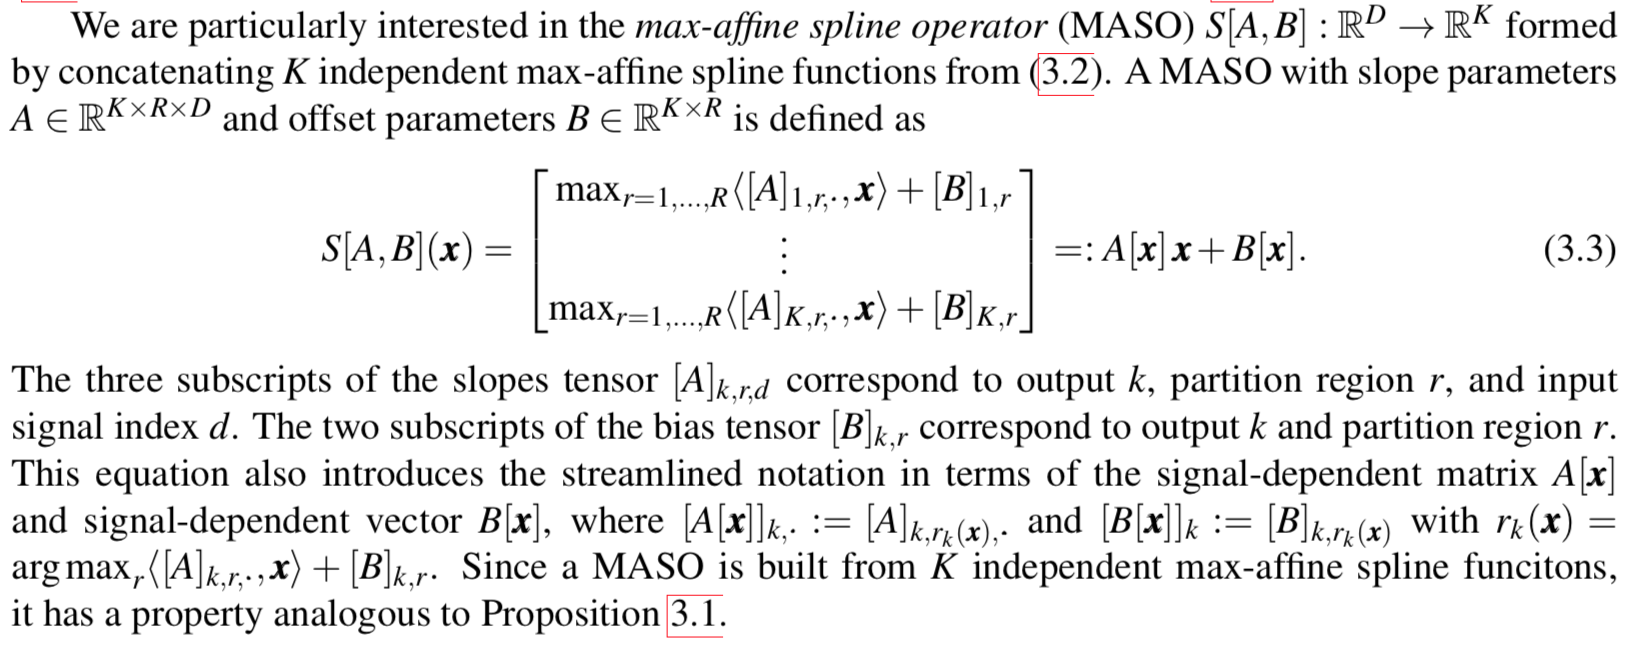
\includegraphics[width=.8\linewidth]{Figure/def_maso}
			\caption{Max-Affine Spline Operators.}
		\label{fig:def_maso}
	\end{center}
\end{figure}

\begin{figure}[h]
\begin{center}
	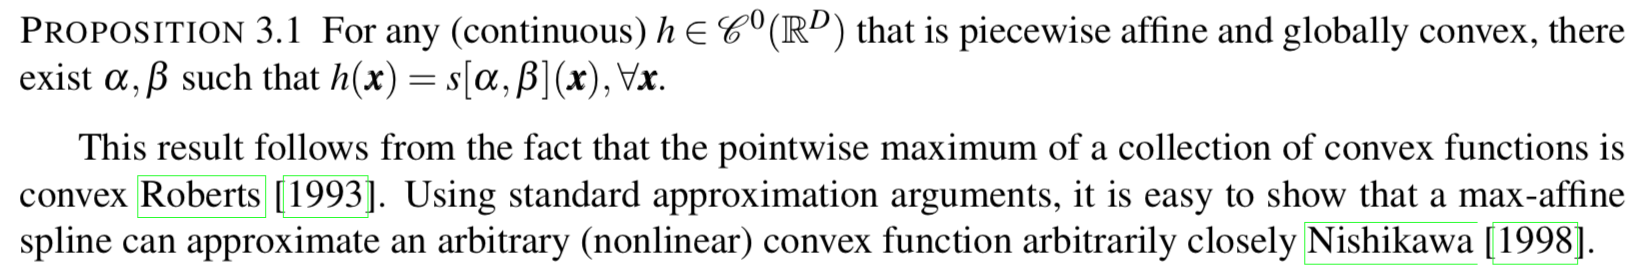
\includegraphics[width=.8\linewidth]{Figure/prop3p1}
%	\caption{xxx}
	\label{fig:prop3p1}
\end{center}
\end{figure}

\begin{figure}[h]
	\begin{center}
		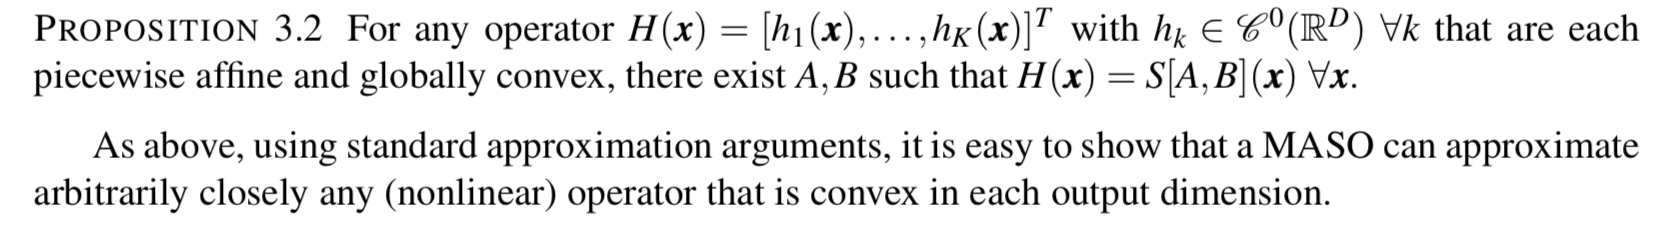
\includegraphics[width=.8\linewidth]{Figure/prop3p2}
		%	\caption{xxx}
		\label{fig:prop3p2}
	\end{center}
\end{figure}


\subsection{Deep Networks are Compositions of Spline Operators}

Proofs in Appendix D. Specifically D.2 which provides MASO forms for layers affine transform + activation, linear skip-connection, ResNet.

\begin{figure}[h]
	\begin{center}
		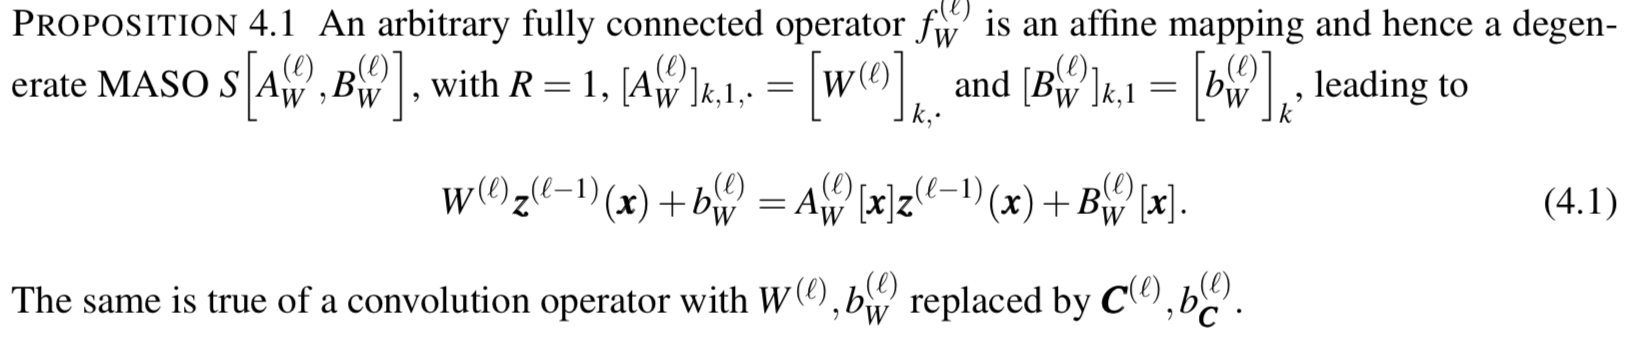
\includegraphics[width=.8\linewidth]{Figure/prop4p1}
		%	\caption{xxx}
		\label{fig:prop4p1}
	\end{center}
\end{figure}

\begin{figure}[h]
	\begin{center}
		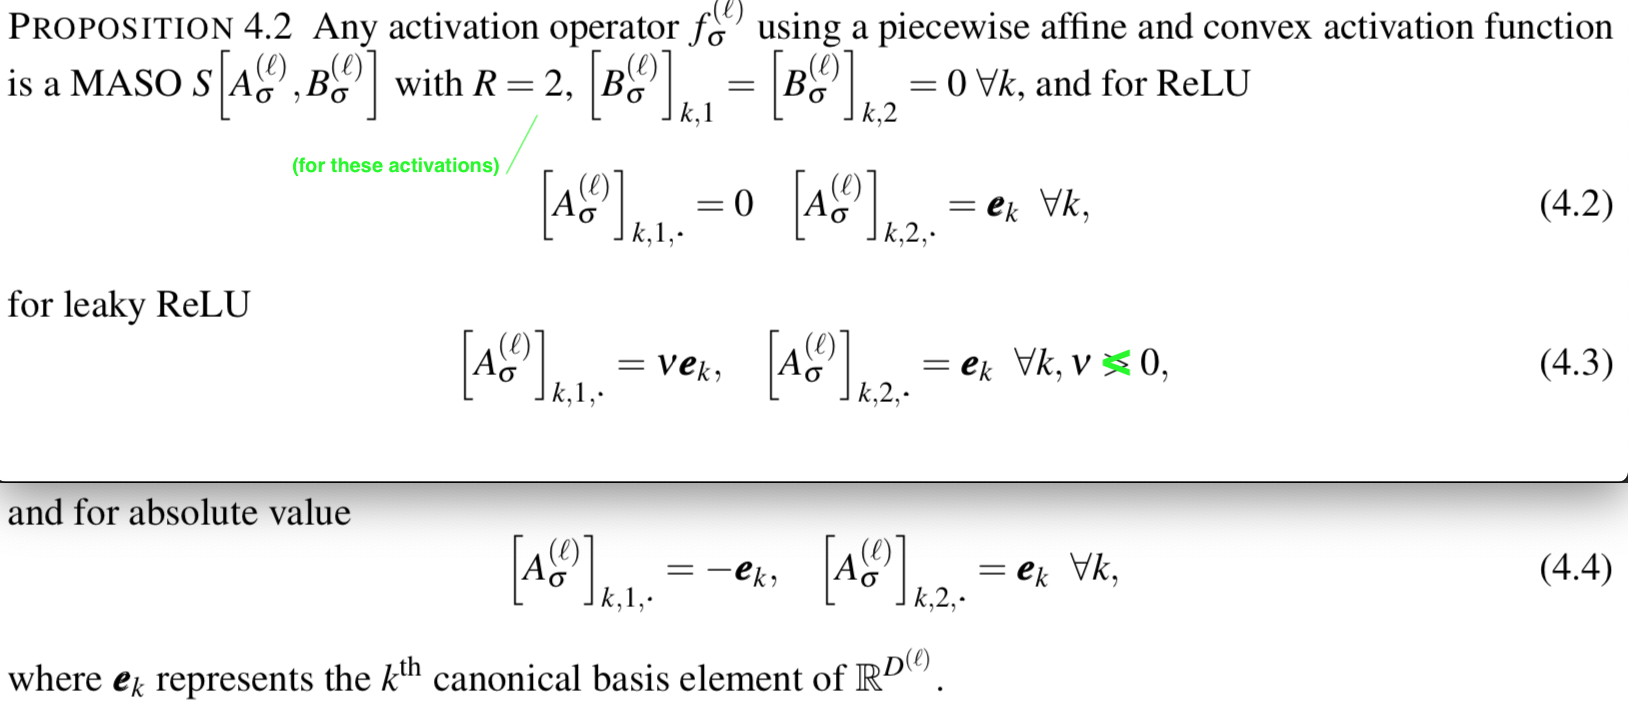
\includegraphics[width=.8\linewidth]{Figure/prop4p2}
		%	\caption{xxx}
		\label{fig:prop4p2}
	\end{center}
\end{figure}


\begin{figure}[h]
	\begin{center}
		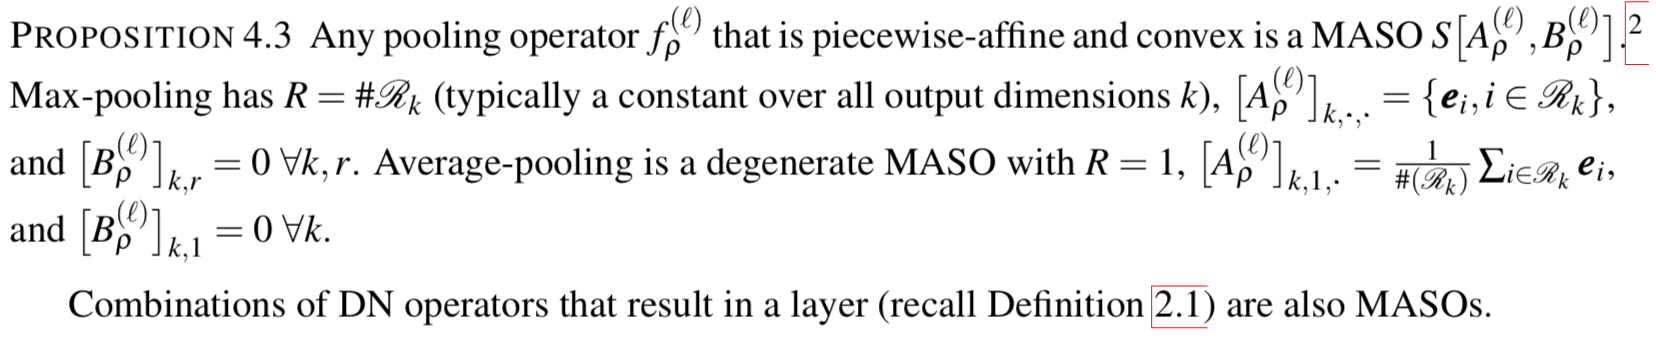
\includegraphics[width=.8\linewidth]{Figure/prop4p3}
		%	\caption{xxx}
		\label{fig:prop4p3}
	\end{center}
\end{figure}

\begin{figure}[h]
	\begin{center}
		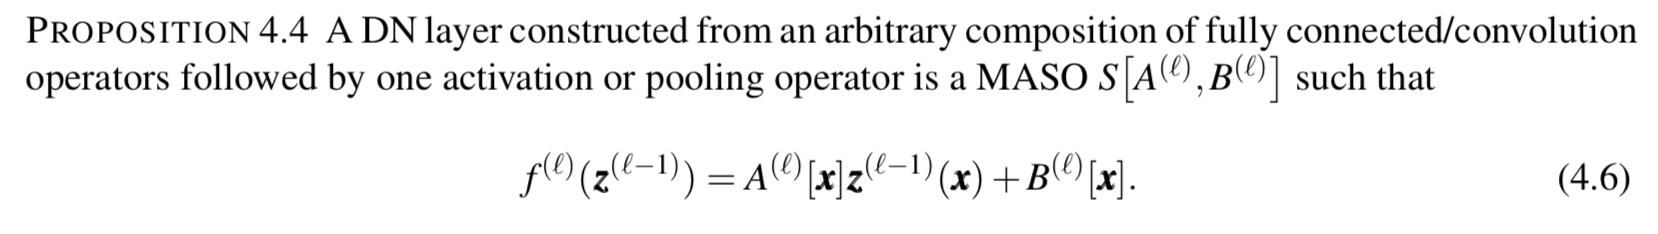
\includegraphics[width=.8\linewidth]{Figure/prop4p4}
		%	\caption{xxx}
		\label{fig:prop4p4}
	\end{center}
\end{figure}


\begin{figure}[h]
	\begin{center}
		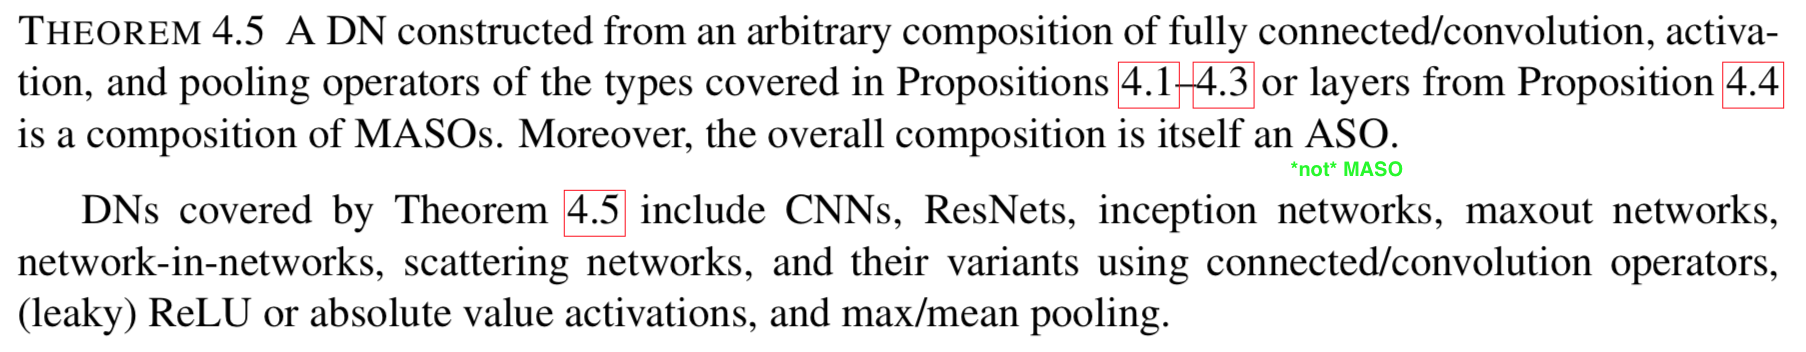
\includegraphics[width=.8\linewidth]{Figure/prop4p5}
		%	\caption{xxx}
		\label{fig:prop4p5}
	\end{center}
\end{figure}

\begin{figure}[h]
	\begin{center}
		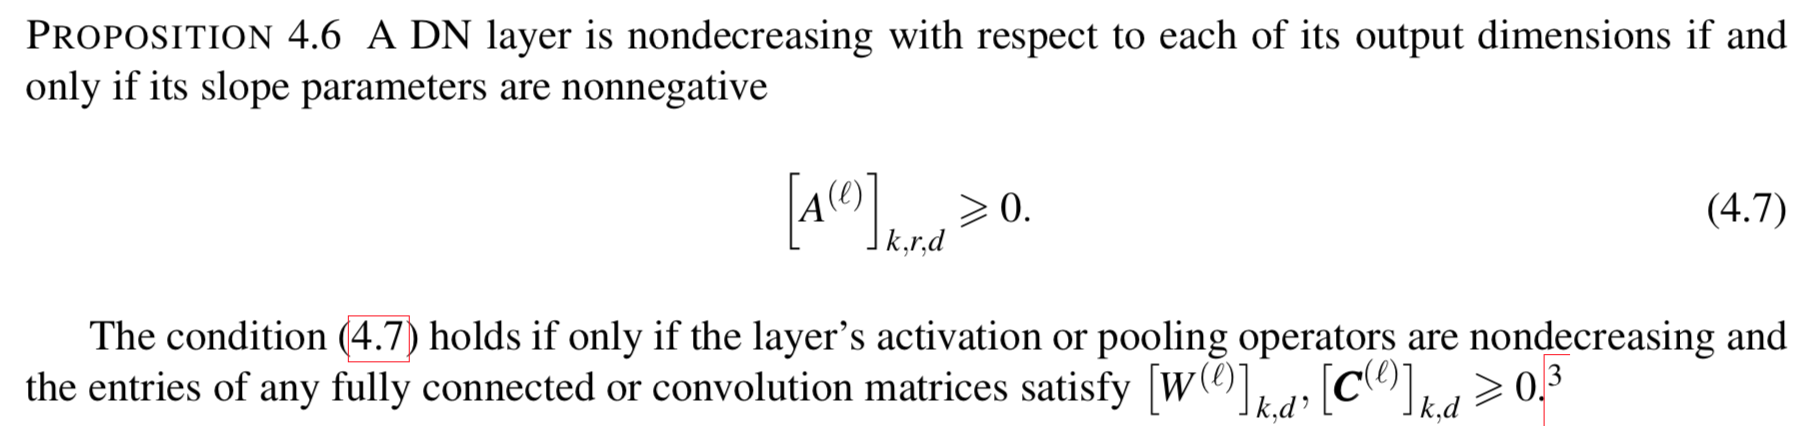
\includegraphics[width=.8\linewidth]{Figure/prop4p6}
		%	\caption{xxx}
		\label{fig:prop4p6}
	\end{center}
\end{figure}

\begin{figure}[h]
	\begin{center}
		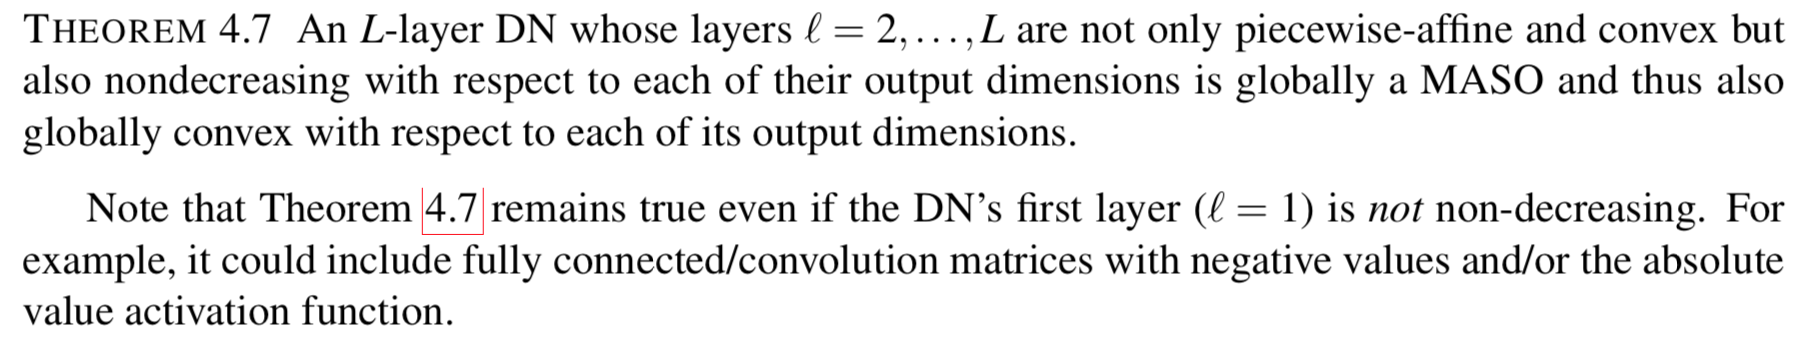
\includegraphics[width=.8\linewidth]{Figure/prop4p7}
		%	\caption{xxx}
		\label{fig:prop4p7}
	\end{center}
\end{figure}


All the beauty of this viewpoint and notations is the fact that it boils down to something close to a linear (affine) transformation, which our minds are ready to handle! More precisely,
\begin{quote}
	The second conclusion in Theorem 4.5 is that the mapping from the input $x$ to the layer output $z^{(l)}(x)$ is an ASO. Hence, $z^{(l)}(x)$ is a \emph{signal-dependent, piecewise affine transformation} of $x$. The particular affine mapping applied to $x$ depends on which partition of the spline it falls in $R^D$.  As such, a more precise but unwieldy terminology that we will not emphasize would be that $z^{(l)}(x)$ is a \emph{partition-region-dependent, piecewise affine transformation} of $x$.
\end{quote}

Examples of formulas for the affine transformations for CNN, ResNet, RNN respectively in sections 4.4, 4.5, Appendix E. These formulations make clear why skip connections stabilize the overall effect of deep CNNs!


\begin{figure}[h]
	\begin{center}
		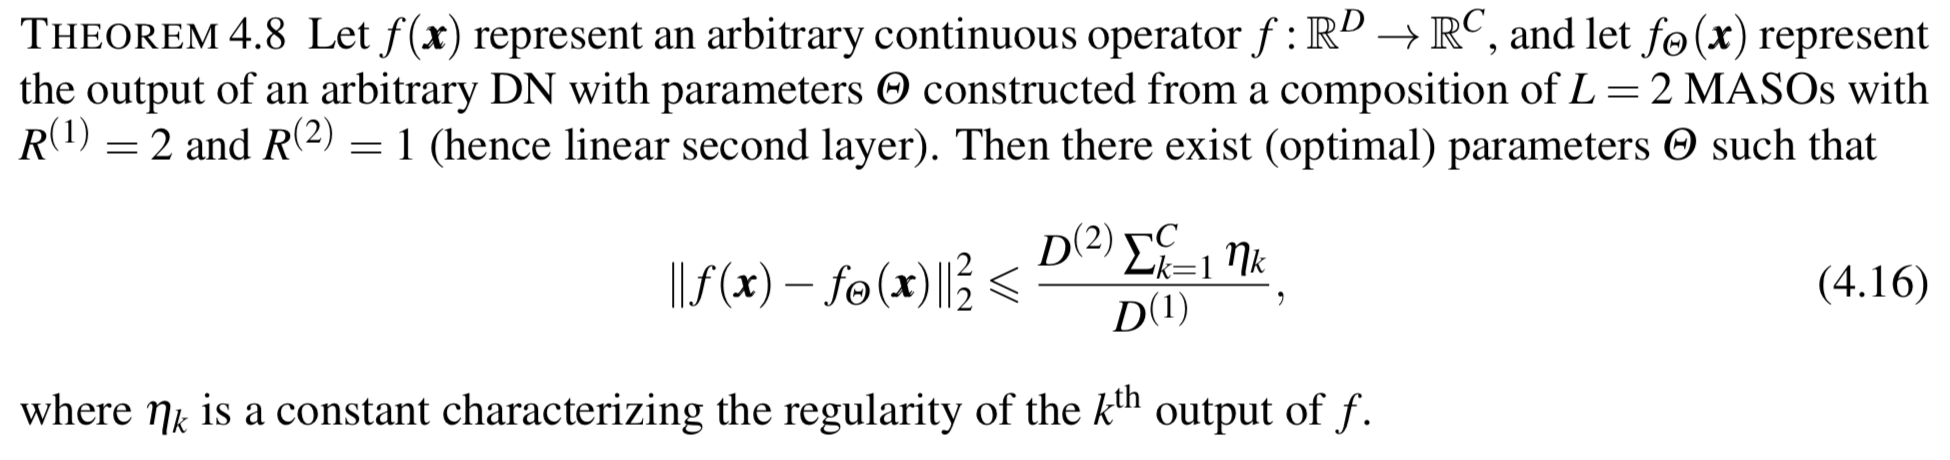
\includegraphics[width=.8\linewidth]{Figure/prop4p8}
		%	\caption{xxx}
		\label{fig:prop4p8}
	\end{center}
\end{figure}



\subsection{DNs are Template Matching Machines}


\begin{figure}[h]
	\begin{center}
		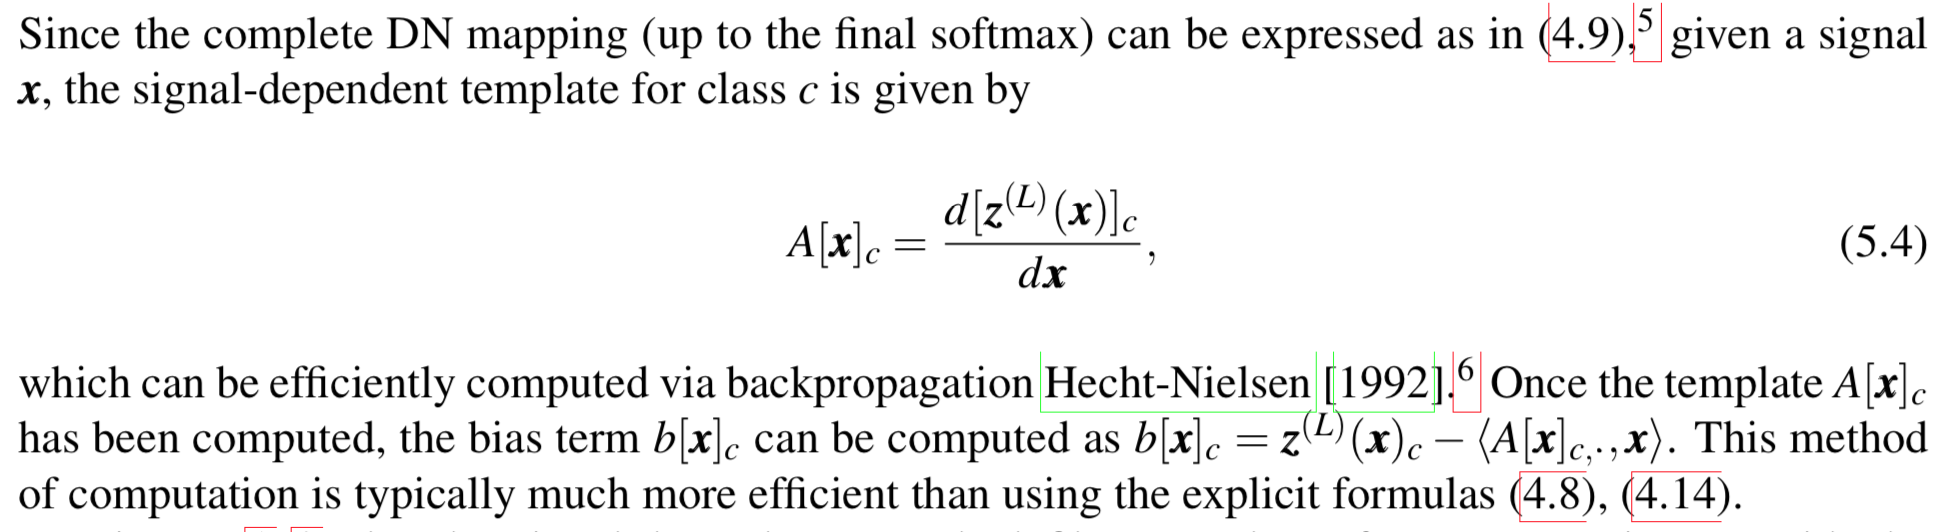
\includegraphics[width=.8\linewidth]{Figure/def_xdeptemplate}
		%	\caption{xxx}
		\label{fig:def_xdeptemplate}
	\end{center}
\end{figure}


The MASO formulation also allows for stability analysis in terms of Lipschitz constants:

\begin{quote}	
	From Proposition 5.3, note the potentially large Lipschitz constants for all operators but the softmax; indeed it is the only contraction, in general. These large constants can reinforce to produce a potentially very large overall Lipschitz constant for the complete DN in (5.9). There are several potential remedies: i) reduce the norms of the fully connected and convolution operators, ii) make the DN narrower by reducing $D^{(l)}$, and iii) invent new, more stable activation and pooling operators.
\end{quote}

\begin{figure}[h]
	\begin{center}
		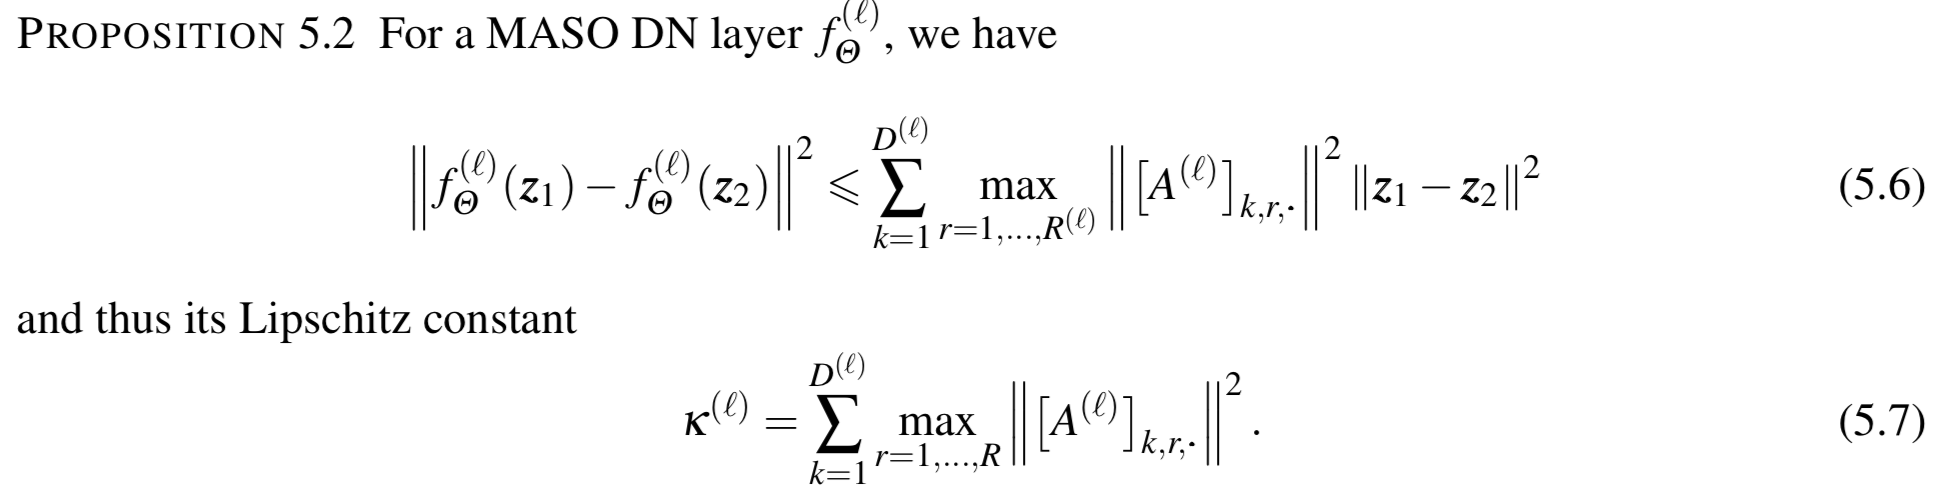
\includegraphics[width=.8\linewidth]{Figure/prop5p2}
		%	\caption{xxx}
		\label{fig:prop5p2}
	\end{center}
\end{figure}

\begin{figure}[h]
	\begin{center}
		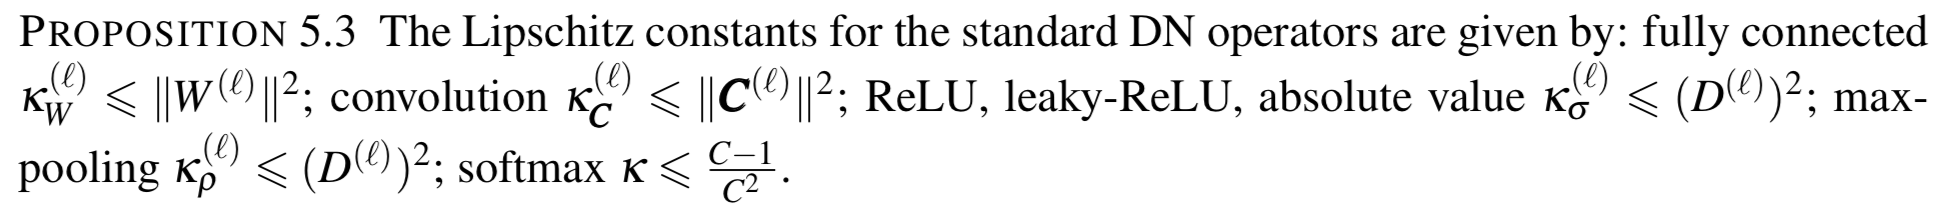
\includegraphics[width=.8\linewidth]{Figure/prop5p3}
		%	\caption{xxx}
		\label{fig:prop5p3}
	\end{center}
\end{figure}


\begin{figure}[h]
	\begin{center}
		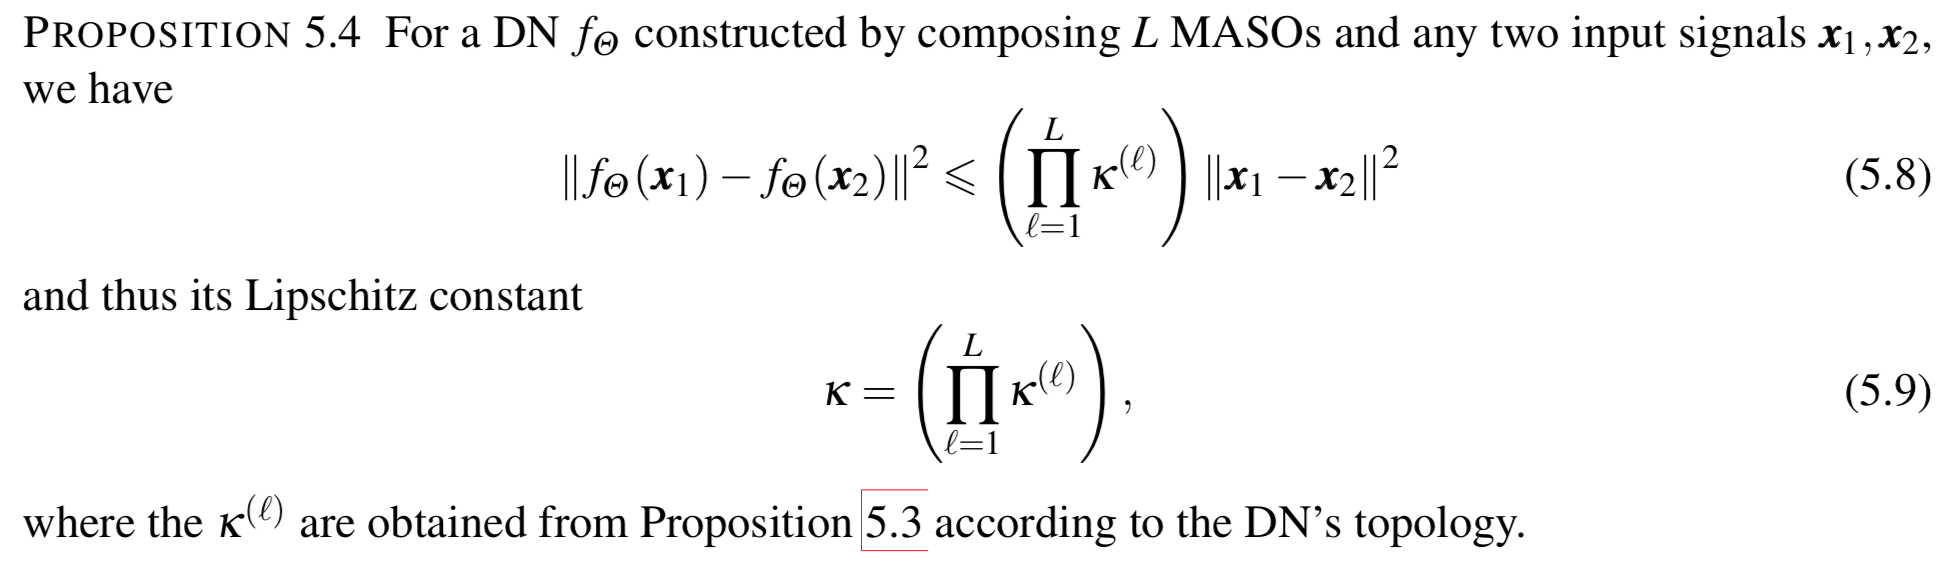
\includegraphics[width=.8\linewidth]{Figure/prop5p4}
		%	\caption{xxx}
		\label{fig:prop5p4}
	\end{center}
\end{figure}


\begin{figure}[h]
	\begin{center}
		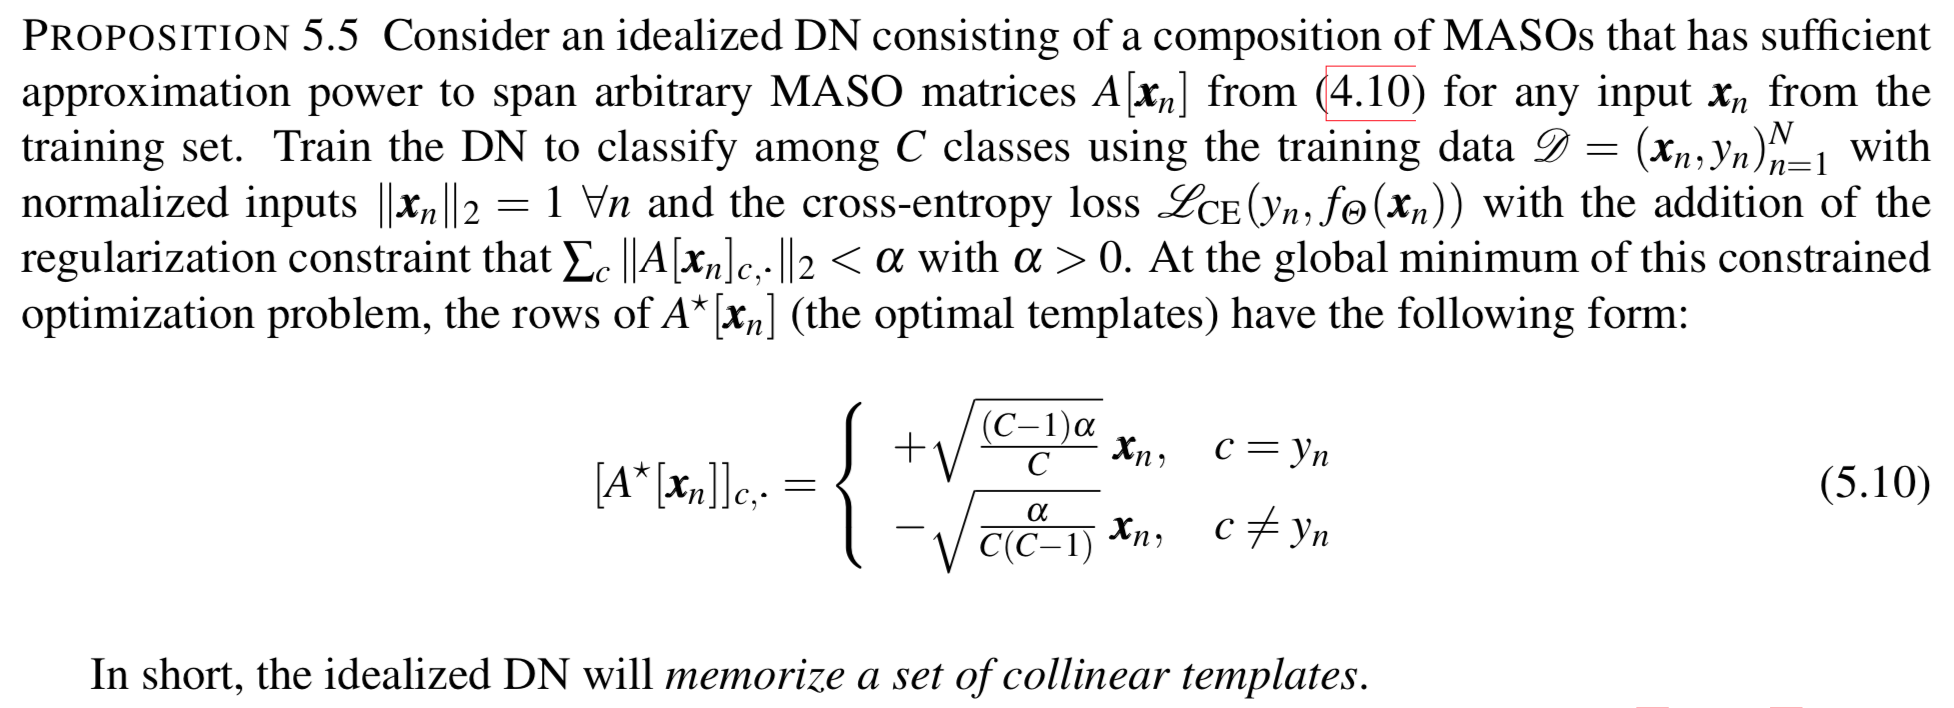
\includegraphics[width=.8\linewidth]{Figure/prop5p5}
		%	\caption{xxx}
		\label{fig:prop5p5}
	\end{center}
\end{figure}



\begin{figure}[h]
	\begin{center}
		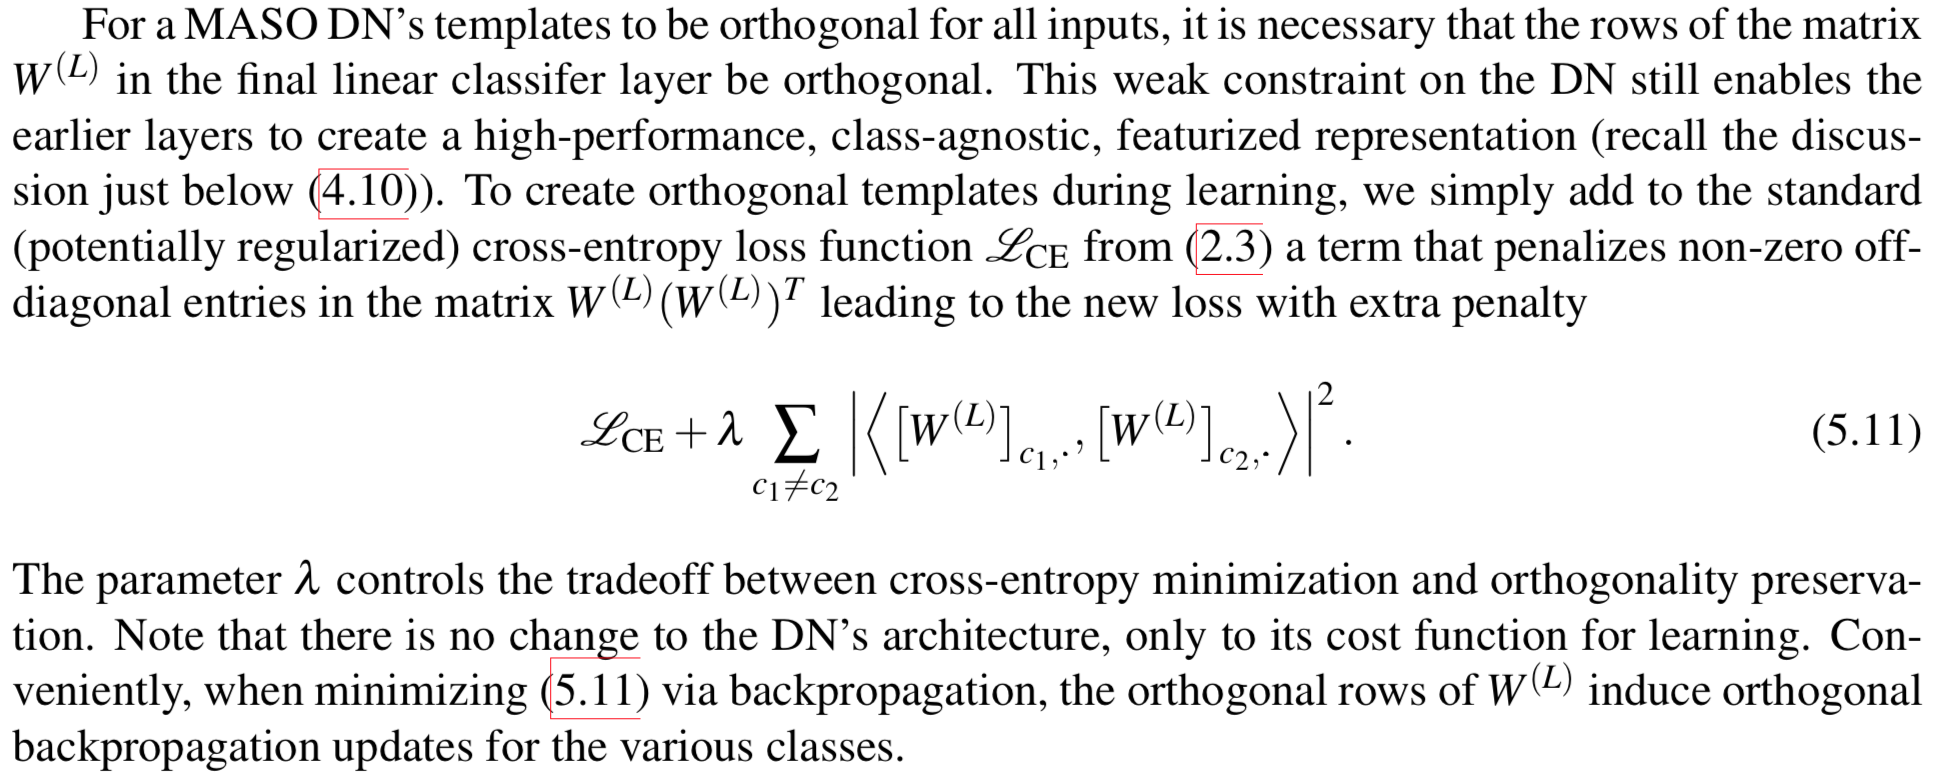
\includegraphics[width=.8\linewidth]{Figure/def_orthotemplatepenalty}
		%	\caption{xxx}
		\label{fig:def_orthotemplatepenalty}
	\end{center}
\end{figure}

\subsection{Multiscale Spline Partition Induced by a DN}

Level $\ell$ of a MASO DN directly partitions its input space $R^{D^{(\ell-1)}}$ and thus indirectly influences the partitioning of the overall input signal space $R^D$ (recall that $ D^{(0)} = D$).\\
The final partition of $R^{D^{(\ell-1)}}$ from a layer-$\ell$ MASO contains up to $ (R^{(\ell)}) ^ {D^{(\ell)}}$ convex and connected regions (in practice, however, many of them could have zero volume).\\
When mapped back to the original input space $R^D$, the partition can be interpreted as a vector quantization of the training data that has been featurized by layers $1$ through $\ell - 1$. Interestingly, the total number of possible regions remains $R^{D^{(\ell-1)}}$. However, the regions are no longer necessarily convex nor connected, due to the nonlinear transformations effected by layers $1$ through $\ell-1$. Moreover, the spline function defined in each region is no longer a fixed affine function; rather it is a piecewise affine function, in general.\\
This input space partition can be plotted using the algorithm described in figure \ref{fig:algo_inputspacepartition}.




\begin{figure}[h]
	\begin{center}
		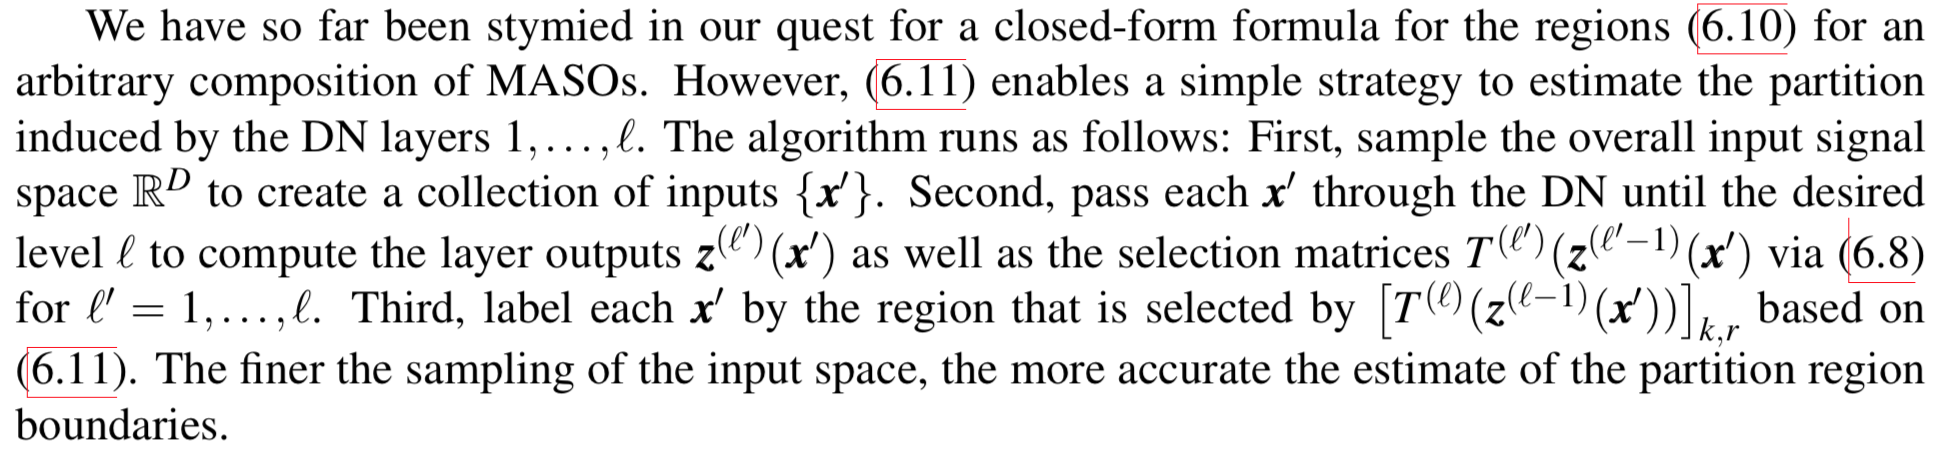
\includegraphics[width=.8\linewidth]{Figure/algo_inputspacepartition}
			\caption{Algorithm to plot input space partitions.}
		\label{fig:algo_inputspacepartition}
	\end{center}
\end{figure}




\begin{figure}[h]
	\begin{center}
		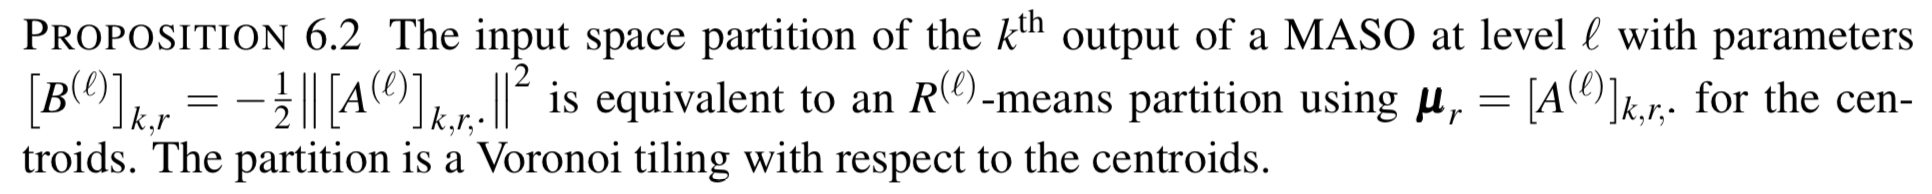
\includegraphics[width=.8\linewidth]{Figure/prop6p1}
%		\caption{Algorithm to plot input space partitions.}
		\label{fig:prop6p1}
	\end{center}
\end{figure}




\begin{figure}[h]
	\begin{center}
		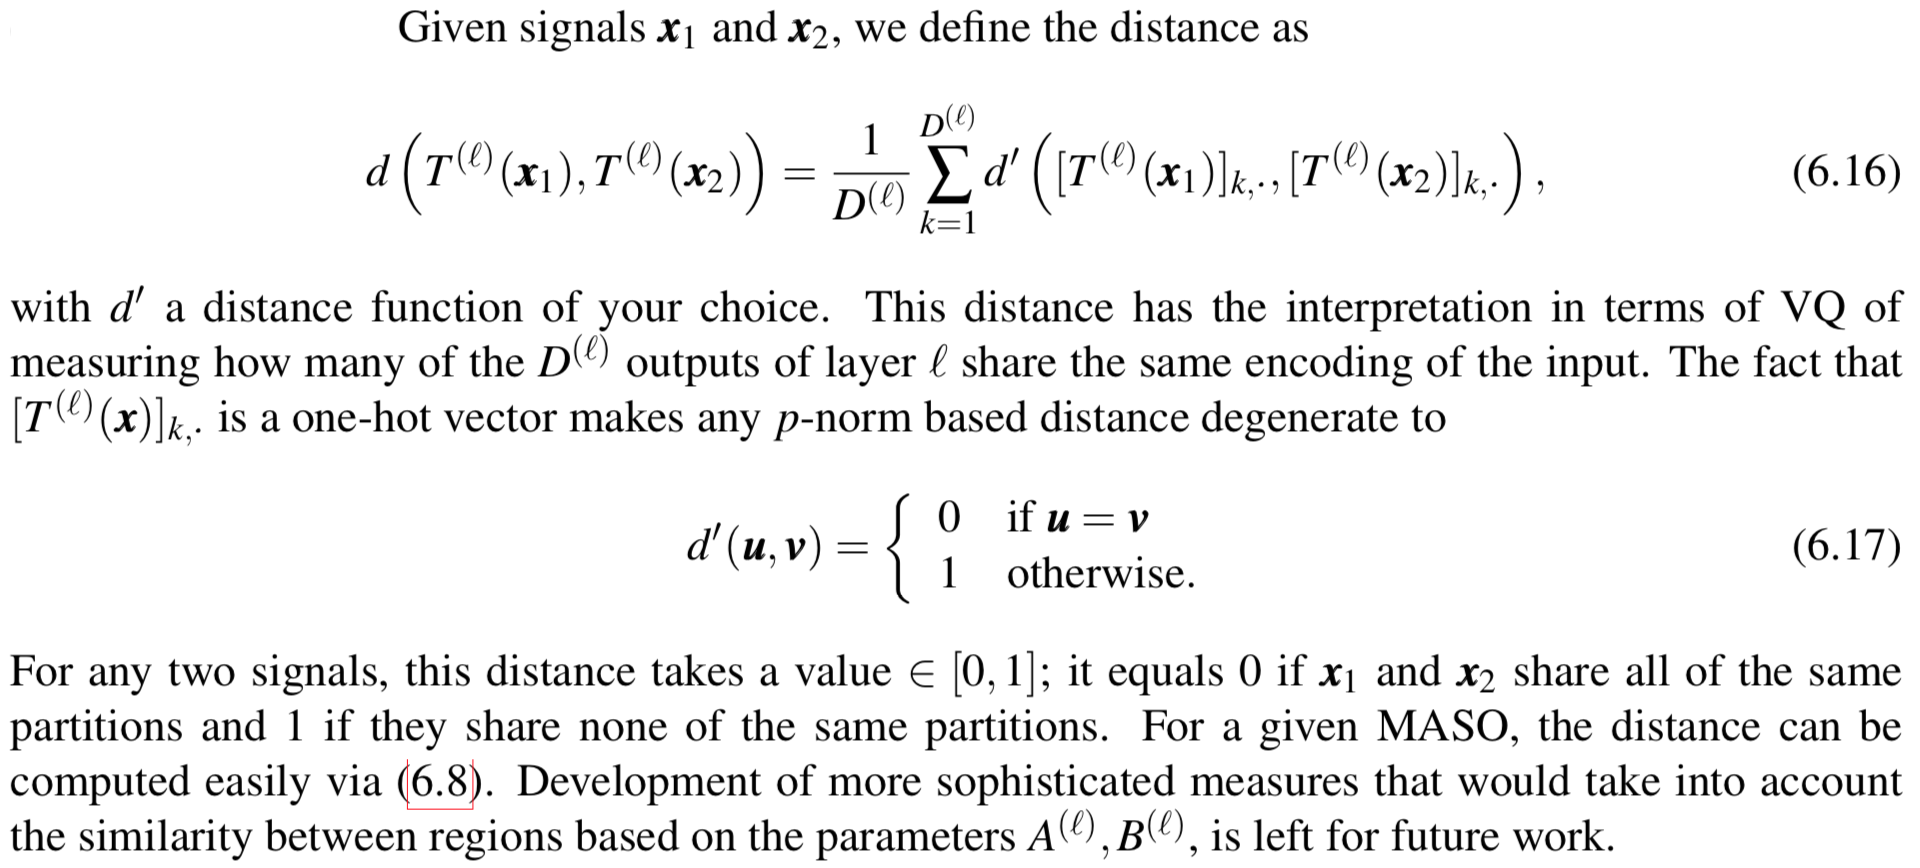
\includegraphics[width=.8\linewidth]{Figure/def_partitionRegionDistance}
		%		\caption{Algorithm to plot input space partitions.}
		\label{fig:def_partitionRegionDistance}
	\end{center}
\end{figure}


The distance (6.16) is defined only with respect to the MASO at level l. However, it is easily extended to take into account the composition of multiple MASO layers by composing their respective selection matrices.


\section{Potential Contributions}

\begin{itemize}
	\item invent new activation and pooling operators that are more stable, in terms of lower Lipschitz constants
	\item extending the NonZero volume / Non Empty partition regions  analysis to the kinds of large DNs used in practice
	\item new constraints on the templates beyond orthogonality could yield learning algorithms that boost performance even further
	\item a deeper study of the spline approximation of non-convex activation functions like the sigmoid could lead to new insights into why they are preferable in certain network topologies (e.g., recursive networks)
\end{itemize}







\bibliographystyle{unsrt}
\bibliography{/Users/arthur/Documents/GitHub/Template_Tex/myLibrary.bib}



\end{document}
